\documentclass[12pt]{letter}
\usepackage{amsmath,amsfonts,amsthm,amstext,amssymb,graphicx, multicol,fancyhdr,lastpage,fullpage,framed,fancybox,enumerate,tikz,color,mathrsfs, polynom, tabto}
\usepackage[margin=0.6in,headsep=3pt, headheight=15pt]{geometry}

% ----------------------------------------------------------
% Custom Definitions, Commands, Environments, etc.

% Sets of numbers
\def\R{\mathbb{R}} % The reals
\def\N{\mathbb{N}} % The naturals
\def\Z{\mathbb{Z}} % The integers
\def\Q{\mathbb{Q}} % The rationals

% Blank space
\newcommand{\blank}[1]{\underline{\hspace{#1}}} % Blank space

% Change font colors
\newcommand{\cyan}[1]{{\color{cyan}{#1}}} % Changes font to cyan
\newcommand{\red}[1]{{\color{red}{#1}}} % Changes font to red
\newcommand{\magenta}[1]{{\color{magenta}{#1}}} % Changes font to magenta
\newcommand{\orange}[1]{{\color{orange}{#1}}} % Changes font to orange
\newcommand{\yellow}[1]{{\color{yellow}{#1}}} % Changes font to yellow
\newcommand{\violet}[1]{{\color{violet}{#1}}} % Changes font to violet
\newcommand{\green}[1]{{\color{green}{#1}}} % Changes font to green
\newcommand{\blue}[1]{{\color{blue}{#1}}} % Changes font to blue
\newcommand{\white}[1]{{\color{white}{#1}}} % Changes font to white

% Fitted inclusion symbols
\newcommand{\fp}[1]{\left({#1}\right)} % Fitted parentheses around content
\newcommand{\fb}[1]{\left[{#1}\right]} % Fitted brackets
\newcommand{\set}[1]{\left\{{#1}\right\}} % Fitted braces (useful for sets)
\newcommand{\av}[1]{\left|{#1}\right|} % Fitted absolute value bars

% Augmented Matrix Environment
\newenvironment{amatrix}[1]{%
	\left[\begin{array}{@{}*{#1}{c}|c@{}}
	}{%
	\end{array}\right]
}

% Miscellaneous
\def\then{\Rightarrow}
\def\to{\rightarrow}
\def\d{^{\circ}}
\newcommand{\?}{\stackrel{?}{=}}



% Coordinate Plane (Four-Quadrant)
\def\coordplane {
	\begin{tikzpicture}		\draw[step=0.25cm,black,very thin,opacity=0.25] (-2.5cm, -2.5cm) grid (2.5cm, 2.5cm);
	\draw[<->,thick,black] (-2.5cm, 0) -- (2.5cm, 0) node[anchor=north west,pos=0.94,font=\scriptsize]{$x$};
	\draw[<->,thick,black] (0,-2.5cm) -- (0, 2.5cm) node[anchor=south east,font=\scriptsize,pos=0.94]{$y$};
	\end{tikzpicture}
}

% Coordinate Plane (One-Quadrant)
\def\onequad {
	\begin{tikzpicture}
	\draw[step=0.25cm, black, very thin, opacity=0.25] (0,0) grid (7.5cm,5cm);
	\draw[->, thick, black] (0,0) -- (7.5cm, 0) node[anchor=north west,font=\scriptsize,pos=0.94]{$x$};
	\draw[->, black, thick] (0,0) -- (0,5cm) node[anchor=south east,font=\scriptsize,pos=0.94]{$y$};
	\end{tikzpicture}
}

% Counters
\newcounter{exercise}

% Exercise environment (auto-numbered)
\newenvironment{exercise}[1][]{\begin{framed}\refstepcounter{exercise}\textbf{Exercise~\theexercise:} #1}{\end{framed}}

% Book exercise environment
\newenvironment{bex}[2][] {
	\begin{framed}
		\textbf{Book Exercise {#2}}#1
	\end{framed}
}
% ----------------------------------------------------------

% ----------------------------------------------------------
% Header and Footer Information
% \pagestyle{fancy}
% \fancyhf{}
% \renewcommand{\headrulewidth}{0pt}
% \rhead{Name: \blank{2in}}
% \lhead{@}
% \rfoot{Page \thepage \, of \,\pageref{LastPage}}
% ----------------------------------------------------------
\author{Jacob Ayers}

\begin{document}
	\textbf{Assignment 4 Key \\ MAT 130}
	
	\begin{bex}{1.7.8}
		{
			
		}
	\end{bex} \vspace{-8pt}
	
	% My answer here
	$2 < x \leq 10$
	
	% \vspace{}
	\vfill % \newpage
	
	\begin{bex}{1.7.22}
		{
			
		}
	\end{bex} \vspace{-32pt}
	
	% My answer here
	\begin{flalign*}
	6x - 4 &\leq 2 + 8x & \\
	-2x &\leq 6 & \\
	x &\geq -3
	\end{flalign*}
	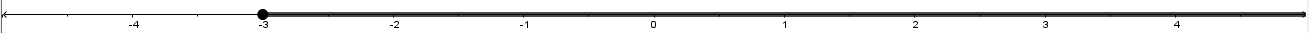
\includegraphics[width=\textwidth]{1722.png}
	
	% \vspace{}
	\vfill % \newpage
	
	\begin{bex}{1.7.34}
		{
			
		}
	\end{bex} \vspace{-32pt}
	
	% My answer here
	\begin{flalign*}
	-1 \leq &-\fp{x - 4} < 7 & \\
	1 \geq & x - 4 \geq -7 & \\
	-7 \leq & x - 4 \leq 1 & \\
	-3 \leq & x \leq 5
	\end{flalign*}
	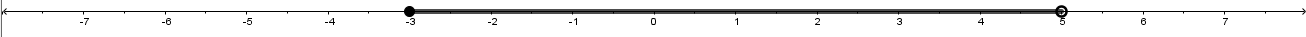
\includegraphics[width=\textwidth]{1734.png}
	
	% \vspace{}
	\vfill % \newpage
	
	\begin{bex}{1.7.42}
		{
			
		}
	\end{bex} \vspace{-32pt}
	
	% My answer here
	\begin{flalign*}
	1.6 < &0.3x + 1 < 2.8 & \\
	0.6 < &0.3x < 1.8 & \\
	2 < &x < 6
	\end{flalign*}
	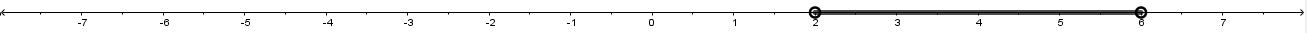
\includegraphics[width=\textwidth]{1742.png}
	
	% \vspace{}
	\vfill \newpage
	
	\begin{bex}{1.7.70}
		{
			
		}
	\end{bex} \vspace{-8pt}
	
	% My answer here
	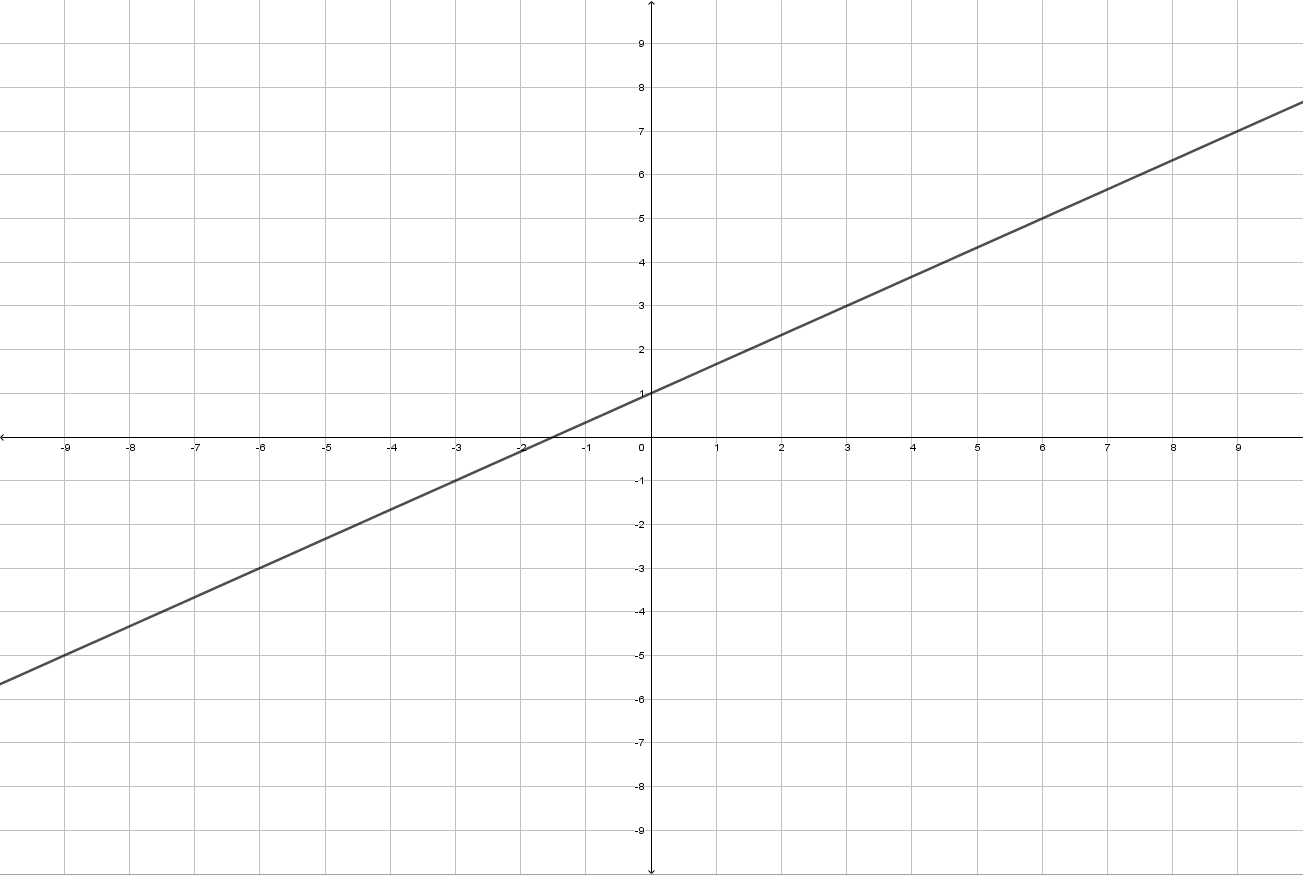
\includegraphics[width=3in]{1770.png}
	
	(a) $(-\infty, 6]$ \\ (b) $[-1.5, \infty)$
	
	% \vspace{}
	\vfill % \newpage
	
	\begin{bex}{1.7.90}
		{
			
		}
	\end{bex} \vspace{-8pt}
	
	% My answer here
	According to the formula, the maximum heart rate is $r = 220 - 40 = 180$ beats per minute. So 50\% of the maximum heart rate is $180\cdot 0.5 = 90$ bpm and 85\% of the maximum heart rate is $180\cdot 0.85 = 153$. So the interval in which a 40-year-old's heart rate is between 50\% and 85\% of max is $[90, 153]$. 
	
	% \vspace{}
	\vfill % \newpage
	
	\begin{bex}{1.7.92}
		{
			
		}
	\end{bex} \vspace{-8pt}
	
	% My answer here
	\underline{Pay Models ($x$ represents number of items produced:} \\
	First job: $13.50$ \\
	Second job: $9 + 0.75x$
	
	We want the second job to pay more. \begin{flalign*}
	9 + 0.75t &> 13.50 & \\
	0.75t &> 4.50 & \\
	t &> 6
	\end{flalign*}
	If you can produce at least 7 items per hour, then the second job will pay more per hour than the first job.
	
	% \vspace{}
	\vfill % \newpage
	
	\begin{bex}{1.7.96}
		{
			
		}
	\end{bex} \vspace{-32pt}
	
	% My answer here
	\begin{flalign*}
	24.55x &> 15.4x + 150000 & \\
	9.15x &> 150000 & \\
	x &>16393.44262
	\end{flalign*}
	You must produce and sell at least 16,394 units in order to return a profit.
	
	% \vspace{}
	\vfill \newpage
	
	\begin{bex}{1.7.102}
		{
			
		}
	\end{bex} \vspace{-8pt}
	
	% My answer here
	(a) We need to find the values of $t$ for which $180 < 3.00t + 163.3 < 190$. \begin{flalign*}
	180 &< 3.00t + 163.3 < 190 & \\
	16.7 &< 3.00t < 26.7 & \\
	5.56 &< t < 9.9
	\end{flalign*}
	Milk production was between 180 billion pounds and 190 billion pounds between 2005 and 2008.
	
	(b) We need to find the values of $t$ for which $3.00t + 163.3 > 230$. \begin{flalign*}
	3.00t + 163.3 &> 230 & \\
	3.00t &> 66.7 & \\
	t &> 22.23
	\end{flalign*}
	Milk production will exceed 230 billion pounds in 2022.
	
	% \vspace{}
	\vfill % \newpage
	
	\begin{bex}{1.8.8}
		{
			
		}
	\end{bex} \vspace{-8pt}
	
	% My answer here
	(a) $\dfrac{3(-2)^2}{(-2)^2 + 4} = \dfrac{12}{8} = 1.5$ \tabto{0.5\textwidth} Not a solution. \\
	(b) $\dfrac{3(-1)^2}{(-1)^2 + 4} = \dfrac{3}{5} = 0.6$ \tabto{0.5\textwidth} Solution. \\
	(c) $\dfrac{3(0)^2}{0^2 + 4} = 0$ \tabto{0.5\textwidth} Solution. \\
	(d) $\dfrac{3(3)^2}{3^2 + 4} = \dfrac{27}{13} \approx 2.08$ \tabto{0.5\textwidth} Not a solution.
	
	% \vspace{}
	\vfill % \newpage
	
	\begin{bex}{1.8.22}
		{
			
		}
	\end{bex} \vspace{-8pt}
	
	% My answer here
	$x^2 + 2x - 3 > 0 \then (x + 3)(x-1) > 0$
	
	Test Intervals: $(-\infty, -3)$, $(-3, 1)$, $(1, \infty)$
	
	\underline{Interval 1: $x = -5$} \\
	$(-5)^2 + 2(-5) - 3 = 25 - 10 - 3 = 12$ \tabto{0.5\textwidth} $+$
	
	\underline{Interval 2: $x = 0$} \\
	$0^2 + 2(0) - 3 = -3$ \tabto{0.5\textwidth} $-$
	
	\underline{Interval 3: $x = 5$} \\
	$5^2 + 2(5) - 3 = 25 + 10 - 3 = 32$ \tabto{0.5\textwidth} $+$
	
	Therefore, the solution is $(-\infty, -3) \cup (1, \infty)$.
	
	
\includegraphics[width=\textwidth]{1822.png}
	% \vspace{}
	\vfill \newpage
	
	\begin{bex}{1.8.26}
		{
			
		}
	\end{bex} \vspace{-32pt}
	
	% My answer here
	\begin{flalign*}
	-2x^2 + 6x + 15 &\leq 0 & \\
	2x^2 - 6x - 15 &\geq 0 & \\
	x &= \dfrac{6 \pm \sqrt{(-6)^2 - 4(2)(-15)}}{2(2)} & \\
	x &= \dfrac{6\pm \sqrt{156}}{4} & \\
	x &= \dfrac{3 + \sqrt{39}}{2} \approx 4.62 & \\
	x &= \dfrac{3 - \sqrt{39}}{2} \approx -1.62
	\end{flalign*}
	Test Intervals: $\fp{-\infty, \dfrac{3 - \sqrt{39}}{2}}$, $\fp{\dfrac{3 - \sqrt{39}}{2}, \dfrac{3 + \sqrt{39}}{2}}$, $\fp{\dfrac{3 + \sqrt{39}}{2}, \infty}$ 
	
	\underline{Interval 1: $x = -2$} \\
	$2(-2)^2 - 6(-2) - 15 = 8 + 12 - 15 = 5$ \tabto{0.5\textwidth} $+$
	
	\underline{Interval 2: $x = 0$} \\
	$2(0)^2 - 6(0) - 15 = -15$ \tabto{0.5\textwidth} $-$
	
	\underline{Interval 3: $x = 5$} \\
	$2(5)^2 - 6(5) - 15 = 50 - 30 - 15 = 5$ \tabto{0.5\textwidth} $+$
	
	Therefore, the solution is $\left(-\infty, \dfrac{3 - \sqrt{39}}{2}\right] \cup \left[\dfrac{3 + \sqrt{39}}{2}, \infty\right)$.
	
	
\includegraphics[width=\textwidth]{1826.png}
	
	% \vspace{}
	\vfill \newpage
	
	\begin{bex}{1.8.36}
		{
			
		}
	\end{bex} \vspace{-8pt}
	
	% My answer here
	$x^4(x-3) \leq 0$
	
	Test Intervals: $(-\infty, 0)$, $(0, 3)$, $(3, \infty)$
	
	\underline{Interval 1: $x = -1$} \\
	$(-1)^4(-1 - 3) = 1(-4) = -4$ \tabto{0.5\textwidth} $-$
	
	\underline{Interval 2: $x = 1$} \\
	$1^2(1 - 3) = 1(-2) = -2$ \tabto{0.5\textwidth} $-$
	
	\underline{Interval 3: $x = 4$} \\
	$4^2(4 - 3) = 16(1) = 16$ \tabto{0.5\textwidth} $+$
	
	Therefore, the solution is $(-\infty, 3]$.
	
	
\includegraphics[width=\textwidth]{1826.png}
	
	% \vspace{}
	\vfill % \newpage
	
	\begin{bex}{1.8.40}
		{
			
		}
	\end{bex} \vspace{-8pt}
	
	% My answer here
	$x^2 - 8x + 16 > 0 \then (x-4)^2 > 0$
	
	Test Intervals: $(-\infty, 4)$, $(4, \infty)$
	
	\underline{Interval 1: $x = 0$} \\
	$0^2 - 8(0) + 16 = 16$ \tabto{0.5\textwidth} $+$
	
	\underline{Interval 2: $x = 5$} \\
	$5^2 - 8(5) + 16 = 25 - 40 + 16 = 1$ \tabto{0.5\textwidth} $+$
	
	This solution set is unusual in that it consists of all real numbers except one. The solution is $x \neq 3$
	
	% \vspace{}
	\vfill % \newpage
	
	\begin{bex}{1.8.58}
		{
			
		}
	\end{bex} \vspace{-8pt}
	
	% My answer here
	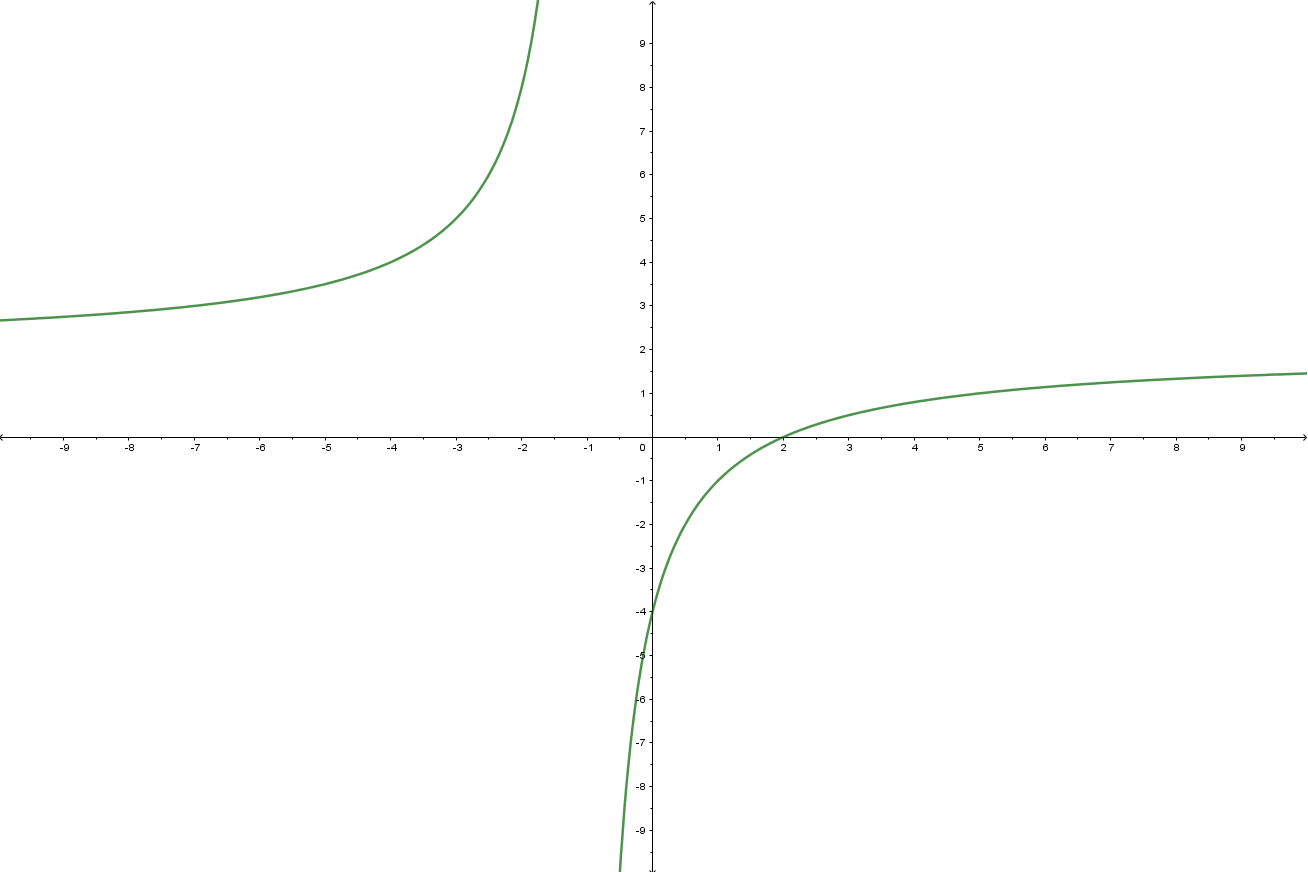
\includegraphics[width=3in]{1858.png}
	
	(a) $(-1, 2]$ \\ (b) $[-2, -1)$ 
	
	% \vspace{}
	\vfill \newpage
	
	\begin{bex}{1.8.68}
		{
			
		}
	\end{bex} \vspace{-8pt}
	
	% My answer here
	(a) \begin{flalign*}
	-16t^2 + 128t &= 0 & \\
	t(-16t + 128) &= 0 & \\
	t &= 0 & \\
	-16t + 128 &= 0 \then t = 8
	\end{flalign*}
	The projectile will be back at ground level 8 seconds after it was fired.
	
	(b) \begin{flalign*}
	-16t^2 + 128t &\leq 128 & \\
	-16t^2 + 128t - 128 &\leq 0 & \\
	t^2 - 8t + 8 &\geq 0 & \\
	t &= \dfrac{8\pm\sqrt{(-8)^2 - 4(1)(8)}}{2(1)} & \\
	t &= \dfrac{8\pm\sqrt{96}}{2} & \\
	t &= 4 + 2\sqrt{2} \approx 6.83 & \\
	t &= 4 - 2\sqrt{2} \approx 1.17
	\end{flalign*}
	Test Intervals: $(0, 1.17)$, $(1.17, 6.83)$, $(6.83, 8)$
	
	\underline{Interval 1: $t = 1$} \\
	$1^2 - 8(1) + 8 = 1 - 8 + 8 = 1$ \tabto{0.5\textwidth} $+$
	
	\underline{Interval 2: $t = 2$} \\
	$2^2 - 8(2) + 8 = 4 - 16 + 8 = -4$ \tabto{0.5\textwidth} $-$
	
	\underline{Interval 3: $t = 7$} \\
	$7^2 - 8(7) + 8 = 49 - 56 + 8 = 1$ \tabto{0.5\textwidth} $+$
	
	So the height will be less than 128 feet for the first 1.17 seconds after the projectile is launched and between 6.83 seconds after launch and the time the projectile hits the ground.
	
	% \vspace{}
	\vfill % \newpage
	
	\begin{bex}{1.8.74}
		{
			
		}
	\end{bex} \vspace{-8pt}
	
	% My answer here
	$49 - x^2 \geq 0 \then x^2 \leq 49$, so the domain is $[-7, 7]$.
	
	% \vspace{}
	\vfill \newpage
	
	\begin{bex}{1.8.78}
		{
			
		}
	\end{bex} \vspace{-8pt}
	
	% My answer here
	(a) Using the table feature of a graphing calculator:
	
	\begin{tabular}{c|ccccc}
		$d$ & 4 & 6 & 8 & 10 & 12 \\ \hline
		Load & 2223.9 & 5593.9 & 10312 & 16378 & 23792
	\end{tabular}

	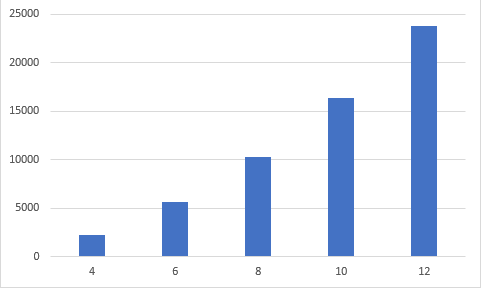
\includegraphics[width=3in]{1878.png}
	
	(b) \begin{flalign*}
	168.5d^2 - 472.1 &= 2000 & \\
	168.5d^2 &= 2472.1 & \\
	d^2 &= 14.67121662 & \\
	d &\approx \pm 3.83
	\end{flalign*}
	So the beam must have a depth of at least 3.84 inches in order to safely support a load of 2000 pounds.
	
	% \vspace{}
	\vfill % \newpage
	
	\begin{bex}{2.1.14}
		{
			
		}
	\end{bex} \vspace{-8pt}
	
	% My answer here
	The slope is $m = -\dfrac67$.
	
	% \vspace{}
	\vfill % \newpage
	
	\begin{bex}{2.1.18}
		{
			
		}
	\end{bex} \vspace{-8pt}
	
	% My answer here
	$m = \dfrac23$, $b = 2$
	
	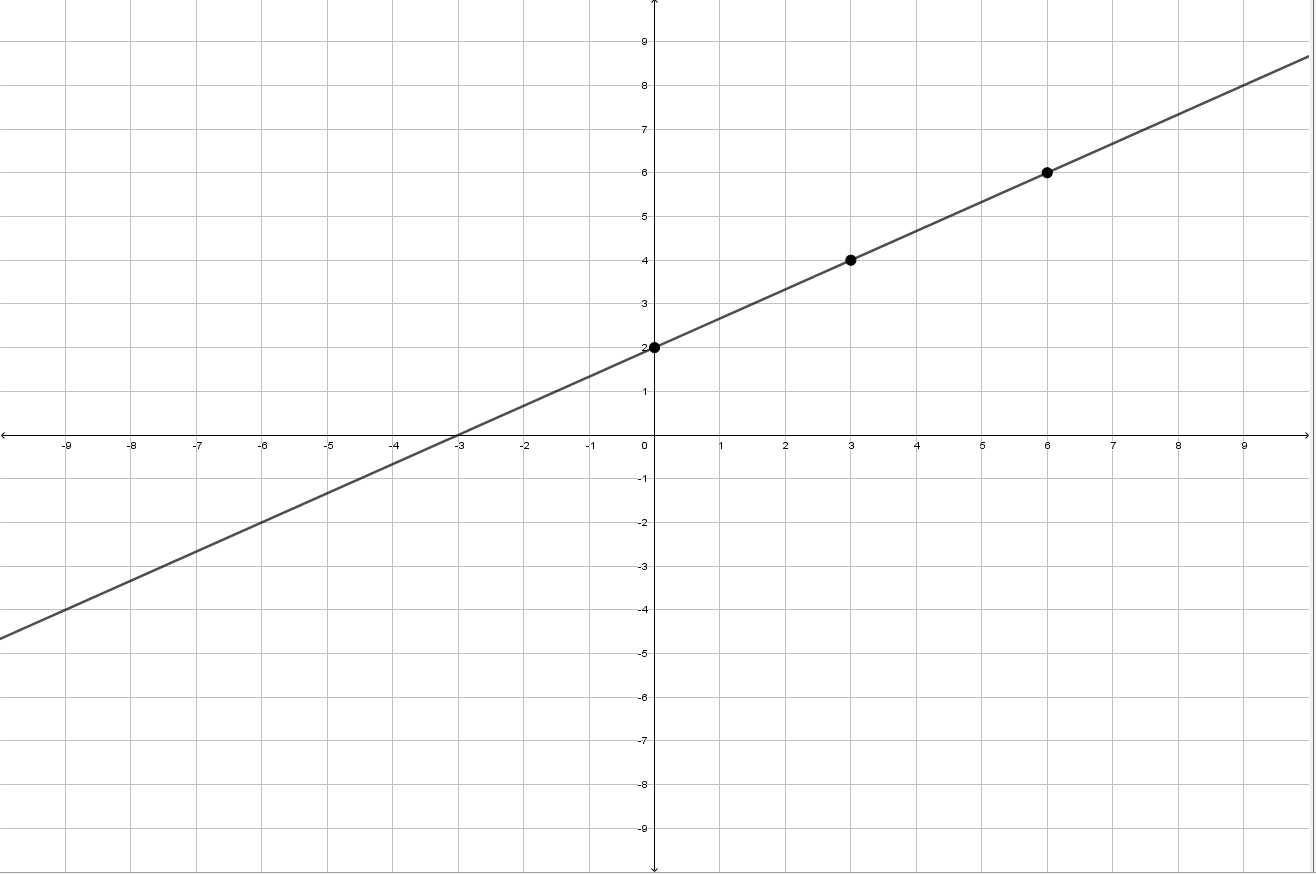
\includegraphics[width=3in]{2118.png}
	
	% \vspace{}
	\vfill \newpage
	
	\begin{bex}{2.1.24}
		{
			
		}
	\end{bex} \vspace{-32pt}
	
	% My answer here
	\begin{flalign*}
	2x + 3y &= 9 & \\
	3y &= -2x + 9 & \\
	y &= -\dfrac23 x + 3
	\end{flalign*}
	$m = -\dfrac23$, $b = 3$
	
	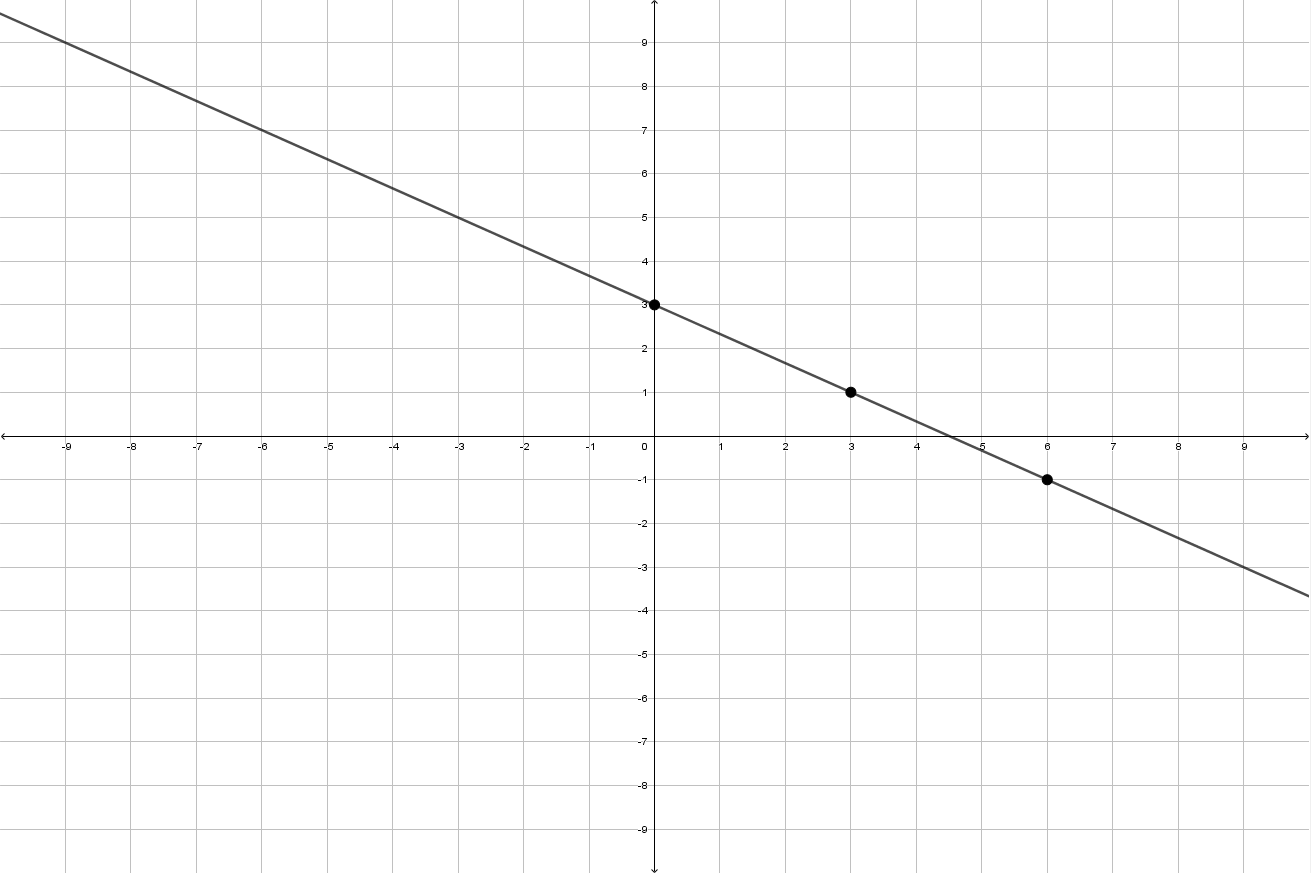
\includegraphics[width=3in]{2124.png}
	
	% \vspace{}
	% \vfill % \newpage
	
	\begin{bex}{2.1.30}
		{
			
		}
	\end{bex} \vspace{-32pt}
	
	% My answer here
	\begin{flalign*}
	m &= \dfrac{y_2 - y_1}{x_2 - x_1} & \\
	&= \dfrac{-5 - 1}{-4 - (-2)} & \\
	&= \dfrac{-6}{-2} & \\
	&= 3
	\end{flalign*}
	
	% \vspace{}
	\vfill % \newpage
	
	\begin{bex}{2.1.38}
		{
			
		}
	\end{bex} \vspace{-8pt}
	
	% My answer here
	There are infinitely many correct answers. To find three of them, we can start at the given point, $(0, -9)$, and use the slope to ``move" and find new ones. The slope tells us that whenever $x$ increases by 1, $y$ will decrease by 2. Using this rule repeatedly yields the following three points.
	
	$(1, -11)$, $(2, -13)$, $(3, -15)$
	% \vspace{}
	\vfill % \newpage
	
	\begin{bex}{2.1.66}
		{
			
		}
	\end{bex} \vspace{-8pt}
	
	% My answer here
	The slopes are $\dfrac14$ and $4$. These numbers are not the same, and they are not opposite reciprocals. So the lines are neither parallel nor perpendicular.
	
	% \vspace{}
	\vfill \newpage
	
	\begin{bex}{2.1.72}
		{
			
		}
	\end{bex} \vspace{-32pt}
	
	% My answer here
	\begin{flalign*}
	m_1 &= \dfrac{2 - 8}{-4 - 4} & \\
	&= \dfrac{-6}{-8} & \\
	&= \dfrac34
	\end{flalign*}
	\begin{flalign*}
	m_2 &= \dfrac{\dfrac13 - (-5)}{-1 - 3} & \\
	&= \dfrac{\dfrac{16}{3}}{-4} & \\
	&= \dfrac{16}{-12} & \\
	&= -\dfrac43
	\end{flalign*}
	These slopes are opposite reciprocals, so the lines are perpendicular.
	
	% \vspace{}
	\vfill % \newpage
	
	\begin{bex}{2.1.74}
		{
			
		}
	\end{bex} \vspace{-8pt}
	
	% My answer here
	Written in slope-intercept form the equation of the given line is $y = -x + 7$ so $m = -1$. Since we aren't specifically asked to give equations in slope-intercept form, we can simply write point-slope equations.
	
	(a) Parallel lines have the same slope, so the equation of the line is $y - 2 = -(x + 3)$.
	
	(b) Perpendicular lines have opposite reciprocal slopes, so th3 equation of the line is $y - 2 = x + 3$.
	
	% \vspace{}
	\vfill % \newpage
	
	\begin{bex}{2.1.96}
		{
			
		}
	\end{bex} \vspace{-8pt}
	
	% My answer here
	We are given two points: $(0, 24000)$ (the y-intercept) and $(10, 0)$. Using these two points, we can easily find the slope and write a slope-intercept equation giving the value $V$ during the 10 years the scanner will be in use.
	\begin{flalign*}
	m &= \dfrac{0 - 24000}{10 - 0} & \\
	&= -2400
	\end{flalign*}
	So, an equation would be $V = -2400t + 24000$.
	
	% \vspace{}
	\vfill \newpage
	
	\begin{bex}{2.1.98}
		{
			
		}
	\end{bex} \vspace{-8pt}
	
	% My answer here
	(a) We are given two points: $(1, 970)$ and $(3, 1270)$. We can find the slope of the line using these points and then write a slope-intercept equation. \begin{flalign*}
	m &= \dfrac{1270 - 970}{3 - 1} & \\
	&= \dfrac{300}{2} & \\
	&= 150 \\
	y - 970 &= 150(x - 1) & \\
	y - 970 &= 150x - 150 & \\
	y &= 150x + 820
	\end{flalign*}
	(b) We saw in part (a) that the slope is 150. This means that, on average, the weight of a male child's brain increases by about 150 grams per year.
	
	(c) $y = 150(2) + 820 = 1120$ g
	
	% \vspace{}
	\vfill % \newpage
	
	\begin{bex}{2.2.8}
		{
			
		}
	\end{bex} \vspace{-8pt}
	
	% My answer here
	The table represents a function since no input is mapped to two different outputs.
	
	% \vspace{}
	% \vfill % \newpage
	
	\begin{bex}{2.2.10}
		{
			
		}
	\end{bex} \vspace{-8pt}
	
	% My answer here
	(a) Not a function since $c$ is mapped to two different outputs. \\
	(b) Is a function from A to B since no input is mapped to two different outputs. \\
	(c) Is a function, but not a function from A to B. It is a function from B to A. \\
	(d) Is a function from A to B since no input is mapped to two different outputs. \\
	
	% \vspace{}
	% \vfill % \newpage
	
	\begin{bex}{2.2.20}
		{
			
		}
	\end{bex} \vspace{-8pt}
	
	% My answer here
	(a) $V(3) = \dfrac43 \pi (3)^3 = \dfrac43 \pi (27) = 36\pi$ \\
	(b) $V\fp{\dfrac32} = \dfrac43 \pi \fp{\dfrac32}^3 = \dfrac43\fp{\dfrac{27}{8}}\pi = \dfrac{9\pi}{2}$ \\
	(c) $V(2r) = \dfrac43 \pi (2r)^3 = \dfrac43 (8r^3) \pi = \dfrac{32\pi r^3}{3}$
	
	% \vspace{}
	\vfill % \newpage
	
	\begin{bex}{2.2.26}
		{
			
		}
	\end{bex} \vspace{-8pt}
	
	% My answer here
	(a) $q(2) = \dfrac{2(2)^2 + 3}{2^2} = \dfrac{11}{4}$ \\
	(b) $q(0)$ is undefined because it results in division by zero. \\
	(c) $q(-x) = \dfrac{2(-x)^2 + 3}{(-x)^2} = \dfrac{2x^2 + 3}{x^2}$
	
	% \vspace{}
	\vfill \newpage
	
	\begin{bex}{2.2.30}
		{
			
		}
	\end{bex} \vspace{-8pt}
	
	% My answer here
	(a) $f(-2) = -3(-2) - 3 = 6 - 3 = 3$ \\
	(b) $f(-1) = (-1)^2 + 2(-1) - 1 = 1 - 2 - 1 = -2$ \\
	(c) $f(1) = 1^2 + 2(1) - 1 = 1 + 2 - 1 = 2$
	
	% \vspace{}
	\vfill % \newpage
	
	\begin{bex}{2.2.42}
		{
			
		}
	\end{bex} \vspace{-32pt}
	
	% My answer here
	\begin{flalign*}
	x^3 - x^2 - 3x + 3 &= 0 & \\
	x^2 (x - 1) - 3 (x - 1) &= 0 & \\
	\fp{x^2 - 3}(x - 1) &= 0 & \\
	x &= \set{-\sqrt{3}, 1, \sqrt{3}}
	\end{flalign*}
	
	% \vspace{}
	\vfill % \newpage
	
	\begin{bex}{2.2.46}
		{
			
		}
	\end{bex} \vspace{-32pt}
	
	% My answer here
	\begin{flalign*}
	\sqrt{x} - 4 &= 2 - x & \\
	\sqrt{x} &= 6 - x & \\
	x &= (6 - x)^2 & \\
	x &= 36 - 12x + x^2 & \\
	x^2 - 13x + 36 &= 0 & \\
	(x - 9)(x - 4) &= 0 & \\
	x &= \set{4, 9}
	\end{flalign*}
	
	% \vspace{}
	\vfill % \newpage
	
	\begin{bex}{2.2.66}
		{
			
		}
	\end{bex} \vspace{-8pt}
	
	% My answer here
	For 2002-2006, use the top equation. For 2007-2011, use the middle equation. For 2012-2014, use the bottom equation. I used the table tool on a graphing calculator to find the following results:
	
	\begin{tabular}{c|c}
		 Years Since 2000, $t$ & Median Sale Price (thousands), $p(t)$ \\ \hline
		 2 & 165.77 \\
		 3 & 182.79 \\
		 4 & 192.29 \\
		 5 & 212.28 \\
		 6 & 224.75 \\
		 7 & 218.37 \\
		 8 & 194.06 \\
		 9 & 177.50 \\
		 10 & 168.70 \\
		 11 & 167.66 \\
		 12 & 177.26 \\
		 13 & 197.32 \\
		 14 & 209.04 \\
	\end{tabular}
	
	% \vspace{}
	% \vfill % \newpage
	
	
\end{document}